\chapter{Introduction}

\section{Base Concepts} \label{sec:base_concepts}

High Performance Computing (HPC), also known as supercomputing, refers to computing systems with extremely high computatiional power that are able to solve hugely complex and demanding problems. \cite{europaHighPerformance}

Often, high precision and accuracy are required in scientific and engineering simulations, which can be achieved by increasing the computational power of the system. This is where HPC comes into play, as it allows for the execution of large-scale \textbf{simulations} of complex problems in a reasonable amount of time. Simulations have become the key method for researching and developing innovative solutions in both scientific and engineering fields. They are especially prominent in leading domains such as the aerospace industry and astrophysics, where they enable the investigation and resolution of highly complex problems. However, the increasing reliance on simulation also introduces significant challenges related to complexity, scalability, and data management, which in turn impact the supporting IT infrastructure.

As scientific inquiry progresses along what is known as the Inference Spiral of System Science, the complexity of models intensifies and the influx of new data enriches these systems with additional insights. Consequently, this dynamic evolution necessitates ever increasing computational power to efficiently handle the enhanced simulations and data management challenges.

\begin{figure}[H]
    \centering
    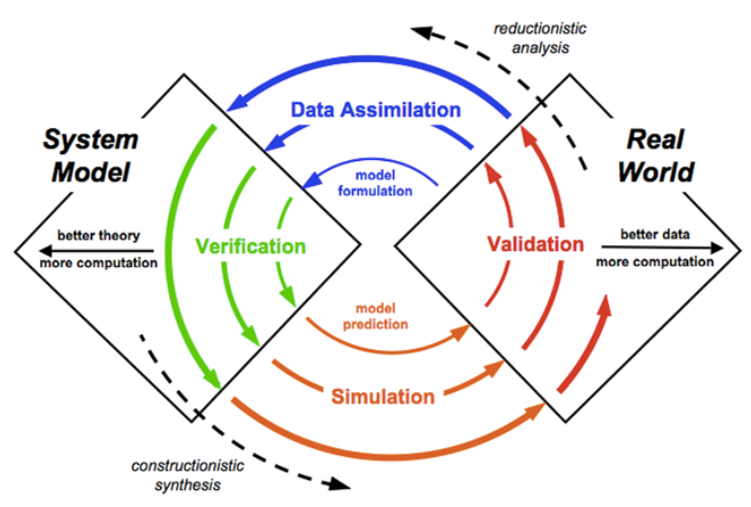
\includegraphics[width=0.55\textwidth]{assets/fig1.png}
    \caption{Research and Development}
    \label{fig:research}
\end{figure}

\begin{observationblock}
In today’s world, larger and larger amounts of data are constantly being generated, from 33 zettabytes globally in 2018 to an expected 181 zettabytes in 2025. This exponential growth is driving a shift towards data-intensive applications, making HPC indispensable for processing and analyzing these vast datasets efficiently. Consequently, HPC is key to unlocking valuable insights that benefit citizens, businesses, researchers, and public administrations. \cite{europaHighPerformance}
\end{observationblock}

\subsection{What is High Performance Computing?} \label{sec:what_is_hpc}

High Performance Computing (HPC) involves using powerful \textcolor{red}{servers, clusters, and supercomputers}, along with \textcolor{blue}{specialized software, tools, components, storage, and services}, to solve computationally intensive \textcolor{ForestGreen}{scientific, engineering, or analytical tasks}. 

HPC is used by scientists and engineers both in research and in production across \textcolor{red}{industry}, \textcolor{blue}{government} and \textcolor{ForestGreen}{academia}.

Key elements of the HPC ecosystem include:
\begin{itemize}
    \item \textbf{\textcolor{red}{Hardware}:} High-performance servers, clusters, and supercomputers.
    \item \textbf{\textcolor{blue}{Software}:} Specialized tools and applications designed to optimize complex computations.
    \item \textbf{\textcolor{ForestGreen}{Applications}:} Scientific, engineering, and analytical tasks that leverage high computational power.
\end{itemize}

\textbf{People in HPC}

Human capital is by far the most important aspect in the HPC landscape. Two crucial roles include HPC providers, who plan, install, and manage the resources, and HPC users, who leverage these resources to their fullest potential. The mixing and interplaying of these roles not only enhances individual competence but also drives overall advancements in high-performance computing.

\subsection{Performance and metrics} \label{sec:performance}

\textbf{Performance} in the realm of high-performance computing is a multifaceted concept that extends far beyond a mere measure of speed. While terms such as “how fast” something operates are often used to describe performance, they tend to be vague. Many factors contribute to the overall performance of a system, and the interpretation of these factors can vary depending on the specific context and objectives of the computational task. Performance, therefore, remains a complex and central issue in the field of HPC, as it involves more than just the raw computational speed.

The discussion often extends to the idea that the "P" in HPC might stand for more than just performance. A growing sentiment among professionals in the field suggests that high performance should be complemented by high productivity. This broader view recognizes that the true efficiency of a computing system is not only determined by its ability to perform tasks quickly but also by the ease and speed with which applications can be developed and maintained. In other words, while raw performance is critical, the overall productivity of a system—combining the system's speed with the programmer's effort—plays an equally important role.

To further clarify the distinction, consider that performance can be seen as a measure of how effectively a system executes tasks, whereas productivity is the outcome achieved relative to the effort invested in developing the application. For instance, if a code optimization leads to a system that runs twice as fast but requires an extensive period of development—say, six months of work—the benefits of the improvement must be weighed against the increased effort required. This example underlines the importance of balancing performance gains with the associated development costs.

Ultimately, the challenge lies in understanding and optimizing both aspects. A successful HPC system is one that not only achieves high computational throughput but also enhances the productivity of the developers who create and refine the applications. This balance is essential for advancing the capabilities of high-performance computing in both research and production environments.

\subsubsection{Number Crunching on CPU} \label{sec:number_crunching}

When evaluating the performance of a high-performance computing (HPC) system, one of the most fundamental metrics is the rate at which floating point operations are executed. This rate is typically expressed in millions (Mflops) or billions (Gflops) of operations per second. In essence, it quantifies how many calculations, such as additions and multiplications, the system is capable of performing every second.

To estimate this capability, we rely on the concept of theoretical peak performance. This value is computed by considering the system’s clock rate, the number of floating point operations that can be executed in a single clock cycle, and the total number of processing cores available. Under ideal conditions, the theoretical peak performance can be expressed as follows:

$$
\text{FLOPS} = \text{clock\_rate} \times \text{Number\_of\_FP\_operations} \times \text{Number\_of\_cores}
$$

This formula provides an upper bound on the computational power of the system. However, it is important to note that this is a best-case scenario estimate and does not always reflect the performance achievable in real applications.

\subsubsection{Sustained (Peak) Performance} \label{sec:sustained}

While the theoretical peak performance offers insight into the maximum potential of an HPC system, the actual performance observed during real-world operations is better captured by the sustained (or peak) performance. In practice, several factors such as memory bandwidth limitations, communication latencies, and input/output overhead can prevent a system from reaching its theoretical maximum.

Sustained performance refers to the effective throughput that an HPC system attains when executing actual workloads. Since it is challenging to exactly measure the number of floating point operations performed by every application, standardized benchmarks are commonly used to assess this performance. One widely recognized benchmark is the HPL Linpack test, which forms the basis for the TOP500 list of supercomputers. This benchmark emphasizes the importance of sustained performance, as it reflects the system’s efficiency and reliability under realistic operational conditions.

Understanding both the theoretical and sustained performance metrics is crucial. While the former provides an idealized estimate of a system's capabilities, the latter offers a more practical perspective, thereby guiding decisions on system improvements and resource allocation in high-performance computing environments.
